% Source: Code/RADAR_web/docs/figures/fig_doppler_byte.tex
\documentclass[border=5pt]{standalone}
\usepackage{tikz}
\usepackage{xcolor}

\definecolor{garnet}{HTML}{73000A}
\definecolor{atlantic}{HTML}{466A9F}

\begin{document}
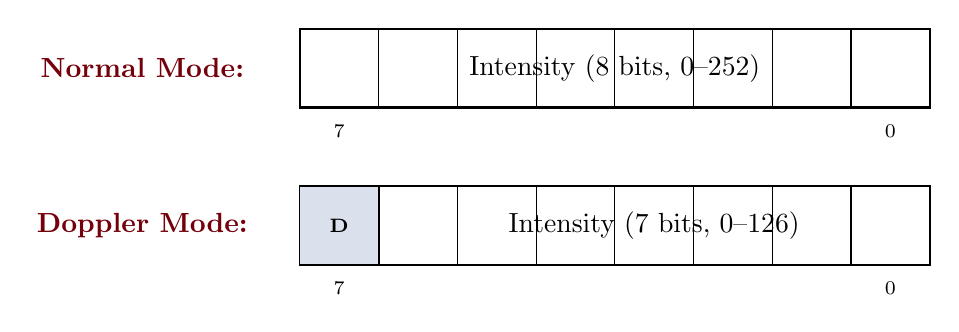
\begin{tikzpicture}
% Normal mode
\node[font=\bfseries\color{garnet}] at (-2, 1.5) {Normal Mode:};
\draw[thick] (0,1) rectangle (8,2);
\foreach \x in {1,...,7} {
    \draw (\x,1) -- (\x,2);
}
\node at (4, 1.5) {Intensity (8 bits, 0--252)};
\node[font=\scriptsize] at (0.5, 0.7) {7};
\node[font=\scriptsize] at (7.5, 0.7) {0};

% Doppler mode
\node[font=\bfseries\color{garnet}] at (-2, -0.5) {Doppler Mode:};
\draw[thick] (0,-1) rectangle (8,0);
\draw[thick] (1,-1) -- (1,0);
\foreach \x in {2,...,7} {
    \draw (\x,-1) -- (\x,0);
}
\draw[fill=atlantic!20] (0,-1) rectangle (1,0);
\node[font=\scriptsize] at (0.5, -0.5) {\textbf{D}};
\node at (4.5, -0.5) {Intensity (7 bits, 0--126)};
\node[font=\scriptsize] at (0.5, -1.3) {7};
\node[font=\scriptsize] at (7.5, -1.3) {0};
\end{tikzpicture}
\end{document}
